\documentclass[fleqn]{jbook}
\usepackage{physpub}

\begin{document}

\begin{question}{教育 物理}{}

% Definition of local macros

\begin{subquestions}
\SubQuestion
  真空中に二つの無限に長い導体の円筒A(半径$a$),およびB(半径$b$)が
  同軸に配置されている。ただし、$a<b$であり、円筒の厚さは無視できる。

  \begin{subsubquestions}
  \SubSubQuestion
    円筒Aに単位長さあたり正電荷$Q$を与え、円筒$B$を接地するとき、
    円筒AとBの間およびBの外側の電場を求め、そのおおよその様子を
    図示せよ。また、二つの円筒間の単位長さあたりの静電容量を求めよ。

  \SubSubQuestion
    円筒の軸方向に一様に電流$I$を流す。電流の向きは円筒AとBで逆向きで
    ある。電流が円筒AとBの間に作る磁束密度を求め、そのおおよその様子
    を図示せよ。また、円筒Aの表面に働く圧力は、
    $\frac{\mu_0I^2}{8\pi^2a^2}$ であることを示せ。ただし、$\mu_0$は
    真空の透磁率である。

  \end{subsubquestions}


\SubQuestion
  図のように、長さ$l$、質量$M$の一様な細い棒の両端がそれぞれ
  水平線($x$軸)上と鉛直線($y$軸)上を離れないように拘束されて滑らかに
  動くようにしてある。棒の重心の座標を$(x,y)$、棒が鉛直線となす角を
  $\theta$とする。\\
%
  \parbox[t]{95mm}{
  \begin{subsubquestions}
  \SubSubQuestion
    棒の中点を通り棒に垂直な軸に関する慣性モーメント$I$は
    $\frac{1}{12}Ml^2$であることを示せ。

  \SubSubQuestion
    力学的全エネルギーを書け。

  \vspace*{2mm}\hspace{-2zw}棒が$x$軸から受ける抗力を$R_y$、$y$軸から受ける抗力を$R_x$とする。

  \SubSubQuestion
    $x$、$y$、$\theta$に対する運動方程式を書け。
  \SubSubQuestion
    設問(ii)で導いたエネルギーが保存することを運動方程式から示せ。

  \vspace*{2mm}\hspace{-2zw}時刻$t=0$で$\theta=0$とし、$\theta$が増す向きに初期角速度$\omega_0$を与えた。

  \SubSubQuestion
    $t\geq 0$での棒の角速度を$\theta$と$\omega_0$で表せ。

  \SubSubQuestion
     $\theta$が小さいとき運動方程式を近似的に解き、$\theta$を時刻$t$
     の関数として与えよ。
  \end{subsubquestions}
  }\parbox[t]{60mm}{
  \begin{center}
    \mbox{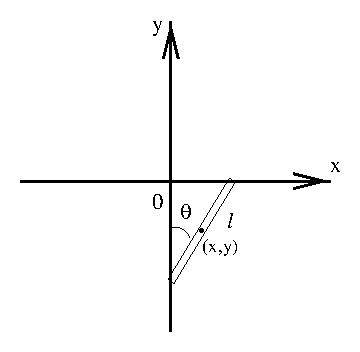
\includegraphics[clip]{1995phys-1.eps}}
  \end{center}}
%


\SubQuestion
  Aさんは、おもちゃ屋でコップの水を飲む動作をいつまでも繰り返す鳥の
  形をしたおもちゃ(次ページの図。{\bf 水飲み鳥}、と呼ぼう)を見つけた。なぜ動力
  も熱の供給もなしに動くかが、すぐにはわからなかったので買い求めて
  調べてみた。まず仕組みは、

  \begin{description}
  \item[(a)]
    本体は、頭と胴にあたる二つの中空のガラス玉を、首にあたる一本の
    ガラス管でつないだ構造である。体内には一部液体が密封されていて、
    外部との液体や空気の出入りは全くない。頭とくちばしの外側は
    フェルトでおおわれており、くちばしに水がつくとフェルトに水が
    しみこむ様になっている。くちばしの内部に隙間はない。ガラス管は、
    頭とは直接つながっているが、胴体には底近くまで深く差し込まれて
    いる。ガラス管の中間にあたる金具の腕を支柱の穴にかけると、支点を
    中心にして前後に回転できる。実際にかけてみたら全身が少し前かがみに
    なるところ({\bf 初期位置}、と呼ぶ)で静止した。(図II-a)。このとき
    液面は胴体の中程にあり、ガラス管内でも同じ高さであった。

  \item[(b)]
    鳥を動かすには、くちばしの部分に水をたっぷりしみこませてから手を
    離して静かに初期位置に置く。しばらくすると胴体内の液体がガラス
    管内をゆっくり上昇して鳥は前に傾き始めた。

  \end{description}
  鳥はその後次ページのような運動をした。

\newpage
  \begin{description}
  \item[(c)]
    傾きがしだいに増して、やがてくちばしがコップの水面に達した(図II-b)
    。さらに傾きが増し、胴体内の液面がガラス管の下端より下がると、
    胴体内の気体の一部がガラス管の中に入り込み、管にそって登りはじめた
    (図II-c)。その結果、ガラス管の中に上昇していた液体が胴体内に落ち
    こみ、ガラス管に上っていった気体と入れ替わった。同時に鳥は水から
    離れ、逆に動きだして、初期位置を通り越すところまで達してから、
    しばらく前後に小さく振動したあと、初期位置より少し前傾した位置で
    ほぼ停止した。この後は、(c)のはじめに戻って、同じ運動をくり返した。
    この反復運動を{\bf 定常水飲み運動}と呼ぶ。ただし、「水飲み動作」
    は、鳥が実際に水を飲むわけではなく、コップの水にくちばしが入って、
    フェルトが濡れるだけである。

  \item[(d)]
    繰り返しの途中でコップを取り去っても、フェルトが濡れている間は
    反復運動を続けるが、しだいに周期が長くなってゆき、フェルトが乾く
    と初期位置で止まった。

  \end{description}
  これだけでは、まだ動く理由がわからないので次のようないろいろな
  実験をした。
  \begin{description}
  \item[(e)]
    気温とコップの水温を測ると、各々$20\degC$と$20\degC$であった。
    コップの水温を下げても、反復運動は続きその周期もあまり変わら
    なかった。しかし、水温を上げていくとくちばしが水中にある時間が
    長くなり、ある温度以上になると反復ののちくちばしを水に入れた状態
    で止まってしまった。

  \item[(f)]
    胴体を手のひらで包むと、ガラス管内の液面はすぐに上昇してたちまち
    頭にまで達した。この際も、また定常水飲み運動の際も、液体の体積
    にはほとんど変化は見られなかった。

  \item[(g)]
    水温と気温がほぼ同じ状態で、コップまで含めた装置全体をすっぽり
    おおうような機密の良い透明な箱をかぶせて観察した。時間がたつと、
    反復時間、特に水中にくちばしを入れている時間がだんだん長くなって、
    何回かの水飲み動作の後、くちばしを水に入れたままもしくは初期位置
    より少し前傾した姿勢のまま完全に止まってしまった。その後おおいを
    静かに取り去ると、すぐに定常水飲み運動に戻った。
  \end{description}
  ここまでの観察と実験で、Aさんは水飲み鳥の作動機構を理解できたという。


  \begin{subsubquestions}
  \SubSubQuestion
    あなたは定常水飲み運動の作動機構をどう理解するか?

  \SubSubQuestion
    上の(d)〜(g)は、あなたの結論に対してどういう根拠を与えたか、
    あるいは、あなたの結論からこれらの観察結果をどう説明できるか?

  \SubSubQuestion
    Aさんは、(g)の状況でさらにある量を測って自分の結論を裏付けた。
    あなたならどういう実験をするか? ((g)の状況に限らず、裏付けと
    なればどんな実験でも良い)その実験から、何を期待し何を実証しよう
    と考えるか?
  \end{subsubquestions}

  \begin{flushleft}
    \hspace{-5mm}\mbox{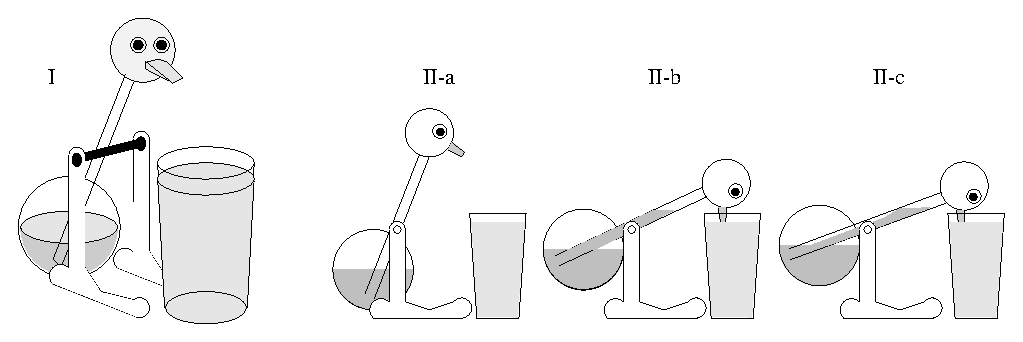
\includegraphics[clip]{1995phys-2.eps}}
  \end{flushleft}

\end{subquestions}
\end{question}
\begin{answer}{教育 物理}{}

% Definition of local macros



\begin{subanswers}
\SubAnswer

  \begin{subsubanswers}
  \SubSubAnswer
    系は軸対称であるから、高さが単位長さの半径$r$の同軸の円柱を積分
    領域に選べば、ガウスの法則より、
%
    \[ (2\pi r \cdot 1)E=\frac{q(r)}{\varepsilon_0} \]
%
    ただし、$q(r)$は、積分領域の中の電荷の総和で、$a<r<b$の時、
    $q(r)=Q$。また、Bの電位が$0$である事から、$r>b$で、$q(r)=0$。
    故に、
%
    \[ E(r) = \left\{\begin{array}{ll}%
                \frac{Q}{2\pi\varepsilon_0 r} & (a<r<b)\\
                0 & (r>b) \end{array}\right. \]
%
    と求まる。\\
%
    次に円筒Aの電位Vは、
%
    \[ V = -\Dint{b}{a}{\d{r}} \frac{Q}{2\pi\varepsilon_0 r}= \frac{Q}{2\pi\varepsilon_0}\ln\frac{b}{a} \]
%
    と求まり、電荷と静電容量との関係が $Q=CV$である事から、
    円筒間の単位長さあたりの静電容量$C$は、
%
    \[ C=\frac{2\pi\varepsilon_0}{\ln(b/a)} \]
%
    と表せる。


  \SubSubAnswer
    系が軸対称であるから、同軸の円周を積分経路に選べば、アンペールの
    法則より、
%
    \[ 2 \pi r B = \mu_0 i(r) \]
%
    ただし、$i(r)$は積分範囲に囲まれる電流の総和で、$a<r<b$で$I$で
    ある。故に、
%
    \[ B(r) = \frac{\mu_0 I}{2\pi r} \]
%
    である。次に仮想的に、Bを固定し、Aの半径が可変で、$r_a$であると
    する。磁場は、AB間にしか存在しないから、空間中の磁場のエネルギー
    $U(r_a)$は、単位長さあたり、
%
    \[ U(r_a) = \frac{1}{2\mu_0}\Dint{r_a}{b}{\d{r}} 2\pi r B(r)^2 %
              = \frac{\mu_0 I^2}{4\pi}\ln\frac{b}{r_a} \]
%
    と求まる。$r_a$を微小量変化させた時に増加する磁場のエネルギーは、
    圧力に抗して加えた仕事に等しく、圧力を$p(r_a)$とすると、
%
    \[ 2\pi r_a p(r_a) = \Deriver{}{r_a}U(r_a) \hspace{15mm} \Yueni p(r_a) = -\frac{\mu_0 I^2}{8\pi^2 r_a^2} \]
%
    よって、圧力は外向きである。

  \end{subsubanswers}



\SubAnswer

  \begin{subsubanswers}
  \SubSubAnswer
    棒の単位長さあたりの質量を$\sigma=M/l$とすると、慣性モーメント
    $I$は、
%
    \[ I = \Dint{-l/2}{l/2}{\d{r}} \sigma r^2 = \frac{1}{12}Ml^2 \]
%
    と表される。

  \SubSubAnswer
    運動エネルギー $T$ は重心の並進運動エネルギーと重心の周りの
    回転運動エネルギーの和である。
%
    \[T=\frac{1}{2}M(\dot{x}^2+\dot{y}^2)+\frac{1}{2}I\dot{\theta}^2 \]
%
    $x,y,\dot{x},\dot{y}$を$\theta,\dot{\theta}$で表すと
%
    \begin{equation}
      x = \frac{l}{2}\sin\theta  \qquad%
      y = -\frac{l}{2}\cos\theta \qquad%
      \dot{x} =  \frac{l}{2} \dot{\theta} \cos\theta \qquad%
      \dot{y} =  \frac{l}{2} \dot{\theta} \sin\theta 
      \eqname{2-1}
    \end{equation}
%
    となるので、これらで$T$を整理すると
%
    \[ T = \frac{1}{6}Ml^2\dot{\theta}^2 \]
%
    と表される。次に位置エネルギー$U$は
%
    \[ U = Mgy = -\frac{1}{2}Mgl\cos\theta \]
%
    と表される。よって、力学的全エネルギー$E$は
%
    
    \begin{equation}
    E = T+U = \frac{1}{6}Ml^2\dot{\theta}^2 - \frac{1}{2}Mgl\cos\theta \eqname{2-2}
    \end{equation}
%
    と表される。


  \SubSubAnswer
    抗力 $R_x,R_y$ は軸と同じ向きに扱うことにする。\\
    重心の並進の運動方程式は以下の通りである。
%
    \begin{equation}
      M\ddot{x} = R_x      \hspace{15mm}%
      M\ddot{y} = R_y - Mg \eqname{2-3}
    \end{equation}
%
    次に回転の運動方程式は以下の通りである。$\theta$の増加方向が、
    普段の$xy$平面とは違うことに注意する。
%
    \begin{equation}
      I\ddot{\theta} = - \frac{l}{2}R_x\cos\theta - \frac{l}{2}R_y\sin\theta \eqname{2-4}
    \end{equation}
%

  \SubSubAnswer
    式\eqhref{2-3},\eqhref{2-4}より抗力 $R_x,R_y$ を消去して整理して
%
    \[ \frac{l}{6}\ddot{\theta} = 
       -\ddot{x}\cos\theta -\ddot{y}\sin\theta -g\sin\theta \]
%
    を得る。右辺の時間微分を次のように変形していく
%
    \begin{eqnarray}
      \frac{l}{6}\ddot{\theta} &=& %
        -\Deriver{}{t} ( \dot{x}\cos\theta + \dot{y}\sin\theta )%
        -\dot{x}\dot{\theta}\sin\theta +\dot{y}\dot{\theta}\cos\theta%
        -g\sin\theta \nonumber \\
      &=& -\Deriver{}{t} \Bigl( \frac{l}{2} \dot{\theta} \Bigr)%
        -g\sin\theta%
        = -\frac{l}{2} \ddot{\theta} -g\sin\theta \nonumber\\
      &\Yueni& 2l\ddot{\theta} +3g\sin\theta = 0 \eqname{2-5}
    \end{eqnarray}
%
    ところで式\eqhref{2-2}のエネルギー$E$を時間微分すると
%
    \[ \dot{E} = \frac{1}{3} Ml^2\dot{\theta}\ddot{\theta}% 
               + \frac{1}{2} Mgl \dot{\theta}\sin\theta%
               = \frac{1}{6}Ml\dot{\theta}(2l\ddot{\theta}+3g\sin\theta) \]
%
     これは式\eqhref{2-5}より$0$である。すなわちエネルギー$E$は
     保存される。


  \SubSubAnswer
    エネルギー$E$が保存されるので$t\geq0$で次の式が成り立つ
%
    \[ \frac{1}{6}Ml^2\dot{\theta}^2 - \frac{1}{2}Mgl\cos\theta = \frac{1}{6}Ml^2\omega_0^2 - \frac{1}{2}Mgl \hspace{10mm}
%
       \Yueni \quad \dot{\theta}^2 = \frac{3g}{l}(\cos\theta -1) + \omega_0^2 \]
%
    棒が鉛直逆立ちになる $\theta=\pi$ のときに $\dot{\theta}$ が
    実数になる場合、つまり $\omega_0 > \sqrt{6g/l}$ の場合には
    棒は原点の周りを回転することになる。他方、逆立ちとなれない場合には
    棒は原点の下を振動することになる。$\dot{\theta}$ は以下の
    通りである。
%
    \[ \dot{\theta} = \left\{ \begin{array}{ll}%
          \ds   +\sqrt{\frac{3g}{l}(\cos\theta -1) + \omega_0^2} &%
          \hspace{15mm}%
          \ds \omega_0 >    \sqrt{\frac{6g}{l}} \mbox{の場合}\\
          \ds \pm\sqrt{\frac{3g}{l}(\cos\theta -1) + \omega_0^2} &%
          \hspace{15mm}%
          \ds \omega_0 \leq \sqrt{\frac{6g}{l}} \mbox{の場合}
       \end{array}\right. \]
%



  \SubSubAnswer
    $\theta \ll 1$に対して $\sin\theta\simeq\theta$と近似すると
    式\eqhref{2-5}は
%
    \[ \ddot{\theta} = -\frac{3g}{2l} \theta \]
%
    となる。この解は明らかに
%
    \[ \theta=\omega_0\sqrt{\frac{2l}{3\raisebox{0.2ex}{$g$}}}\sin\sqrt{\frac{3g}{2l}}t \]
%
    である。

  \end{subsubanswers}



\SubAnswer

  \begin{subsubanswers}
  \SubSubAnswer
    くちばしについた水が蒸発することにより、気化熱を奪い、頭部が胴体
    よりも冷える。頭部では、凝結が起こり、蒸気圧が下がる。すると、
    胴体内と頭部の圧力差により、管を液体が上昇する。すると、重心が
    移動して、水飲み鳥は前傾して、くちばしをぬらす。同時に、体内の
    液体の量とガラス管の位置が上手く調整してあるため、水を飲んでいる
    状態で、胴体内の気体が管内を通って頭部へ上昇し、頭部の液体を胴体
    に戻すと同時に、気圧差を解消する。このようにして、水飲み鳥は、
    再び立ち上がる。以後、この動作を繰り返す。

  \SubSubAnswer
    (d)は、この作動機構は、くちばしが濡れていることが重要であり、
    コップとその中の水の存在は本質的なものでないことを示していて、
    (i)の作動原理の理解に矛盾しない。\\
    (e)は、頭部が胴体よりも冷えていることが本質的であることを示して
    いる。これも(i)の作動原理の理解に矛盾しない。\\
    (f)は、体積の変化がほとんど無いのに、手で胴体を包むと液体が
    上昇したので、液体の上昇は、胴体が暖められて、胴体内の気体の
    圧力が上昇して、液体を持ち上げたためと考えられる。その際、
    もしそれが、気体の体積膨張によるものなら、高々、$\Delta T/273$
    程度の割合しか上昇しない。むしろ、胴体には揮発性の高い液体が
    入っていると考えるほうが合理的である。数度の変化で蒸気圧が大きく
    変わる事を考えれば、頭部と胴体が数度の温度差しか無くても、多くの
    液体を動かすことができて、水飲み鳥を動かすことができると考えら
    れる。これにより、水飲み鳥の動作原理を推測できる。\\
    (g)はくちばしの水分の蒸発が運動を支えていることを示している。
    蒸発することにより、気化熱を奪うので、頭部に低温熱源があること
    になる。これから、胴体部分が頭部に比べて高温であることから、
    熱力学的に仕事が生まれることが説明できる。仕事率は二つの熱源の
    温度差に比例していて、それはくちばしからの蒸発量による。これは、
    水飲み鳥をおおうと、しだいに動きがゆっくりになっていったことを
    良く説明している。\\


  \SubSubAnswer
    頭部と胴体に0.1度程度まで分かる温度計(熱電対)を、水飲み鳥の動作
    に支障が出ないように取り付け、水飲み鳥の動作状況と温度変化を観察
    する。覆いがしてあり、中に水があれば、しだいに内部は飽和蒸気圧に
    達する。よって、時間経過とともに、頭部と胴体の温度差の一動作周期
    あたりの最大値が小さくなるはずである。また、それに伴って、動作の
    周期が延びるはずである。それらの関係を実証する。

  \end{subsubanswers}
\end{subanswers}
\end{answer}


\end{document}
